\section{Trames LoRaMAC}\label{sec:archi-loramac-frame}
\renewcommand{\rightmark}{Trames LoRaMac}

    Le protocole MAC mis en place pour les communications LoRa utilise un seul format de trames illustré à la figure~\ref{fig:archi-frame}.
    \begin{figure}[H]
        \centering
        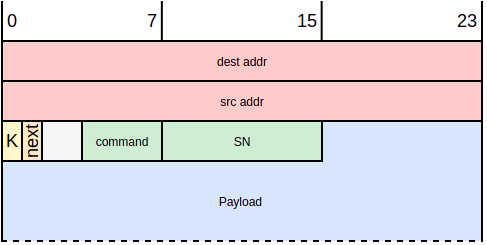
\includegraphics[scale=0.5]{res/pictures/loramac-frame.drawio.png}
        \caption{Format de trame LoRaMAC.}
        \label{fig:archi-frame}
    \end{figure}
    Les trames LoRaMAC sont composées des champs suivants:
    \begin{itemize}
        \item \textbf{dest\_addr}: l'adresse de destination (24 bits)
        \item \textbf{src\_addr}: l'adresse source (24 bits)
        \item \textbf{K}: un flag  qui indique si la trame nécessite un acquittement (1 bit)
        \item \textbf{next}: un flag qui indique si une autre trame suit (1 bit)
        \item \textbf{reserved}: 2 bits non utilisés
        \item \textbf{command}: la commande MAC (4 bits).\\
        Les commandes disponibles ainsi que leurs valeurs sont reprises dans la table~\ref{tb:archi-loramac-command}
        \item \textbf{SN}: le numéro de séquence de la trame (8 bits)
        \item \textbf{Payload}: la payload ayant un MTU de 247 octets
        \begin{table}[H]
            \centering
            \begin{tabular}{|c|c|}
                \hline
                Valeur & Commande\\ \hline
                0 & JOIN\\ \hline
                1 & JOIN\_RESPONSE\\ \hline
                2 & DATA\\ \hline
                3 & ACK\\ \hline
                3 & QUERY\\ \hline
            \end{tabular}
            \caption{Commandes LoRaMAC.}
            \label{tb:archi-loramac-command}
        \end{table}
    \end{itemize}
